% !Mode:: "TeX:UTF-8"

\documentclass{zjutthesis}

\graphicspath{{figures/}}  % 定义所有的eps文件在 figures 子目录下
\begin{document}           % 开始全文

%论文题目:{中文}
\zjuttitle{基于内存数据库的大数据应用系统的设计与实现}
%作者:{中文姓名}{学号}
\zjutauthor{陈佳鹏}{20092663503}
%指导教师:{导师中文名}
\zjutmentor{陈~~~~波}
%个人信息:{毕业年份}{专业名称}
\zjutinfo{2013}{软件工程}
%学院信息:{学院中文}
\zjutcollege{计算机科学与技术学院}
%日期:{提交日期}
\zjutdate{2013年06月}

% !Mode:: "TeX:UTF-8"
%%============================================================
%% 中文封面
\thispagestyle{empty}
\pdfbookmark[-1]{\zjuttitlec}{zjutreportcover}
\phantomsection \label{zjutreportcover}
\vspace*{-2.5mm}
% 校名
\begin{center}
   
\includegraphics[width=98.40mm]{figures/zjut}
\end{center}
\vspace*{9.66mm}
\centerline{\songti\yihao{\reporttitle}}
\vspace*{10.0mm}
\centerline{\heiti\xiaoer\textbf{(\zjutgrade\ 届)}}
\vspace*{8.5mm}
% 校徽
\begin{center}
  
\includegraphics[width=27.3mm]{figures/zjutlogo}
\end{center}

\vspace*{0.0mm}
\renewcommand{\arraystretch}{1.0}
\hspace*{7.4mm}
{\songti\erhao{论文题目}}
\hspace{6mm}
\begin{minipage}[t]{95mm}
    \linespread{1.1}{\songti\xiaoer\uline{\zjuttitlec}}
\end{minipage}
\vspace*{9mm}
\begin{center}
    \setlength{\arrayrulewidth}{0.5pt}
    {\songti\sihao
        \renewcommand{\arraystretch}{1.4}
        \begin{tabular}{lc}
            作者姓名 \qquad &  \zjutauthornamec \\ \cline{2-2}
            指导教师\qquad &  \zjutmentorc\\ \cline{2-2}
            \\
            学科(专业)\qquad &  \zjutmajor \\ \cline{2-2}
            所在学院\qquad &  \zjutcollegec \\ \cline{2-2}\cline{2-2}
            提交日期\qquad & \zjutsubmitteddatee \\ \cline{2-2}
        \end{tabular}
    }
\end{center}

      % 封面

\frontmatter

\pagenumbering{Roman}
% !Mode:: "TeX:UTF-8"
%% 中文摘要
\begin{abstractc}
随着互联网的高速发展,各种大数据类型的应用层出不穷。低延迟I/O等高需求的条件对传统的磁盘数据库产生了很大冲击。内存数据库是最近很热门的技术,它将数据完全放在内存中,而传统的硬盘只用做数据库的持久化备份,使得应用程序对数据有极高的处理速度。

本文基于Redis及SQLite等开源数据库,实现了一个大数据的应用系统,重点对Redis底层数据结构的设计原理及方法进行了分析。使用Python语言编写了主要功能的模块,其中GUI部分基于扩展库PyQt4开发。为方便用户使用,本系统在Redis原命令的基础上实现了一些基础的SQL操作(Create,Select 等),并能够在GUI中显示相应的操作结果。在性能测试方面,重点对数据读取性能与热门的关系型数据库MySQL(5.5)进行了对比,比较了两者在读写速度上的差异。

实验结果表明,本系统实现了内存数据库的基本操作。与磁盘数据库相比,在读写性能上有较大的提高,可以满足数据挖掘大数据应用的需求。


% 摘要内容,小四号宋体,段前段后0磅,1.5倍间距。500字左右。每段开头空两格,标点符号占一格。中文摘要应表达毕业设计工作的核心内容,简短明了。
% 首先,摘要应当要素齐全。即一篇摘要应当包含如下要素:
% 1.目的—即从事该项研究开发的理由与背景或所涉及的主题范围;
% 2.方法—即所用的原理﹑理论﹑开发工具,关键技术解决方法等;
% 3.结果—即研究开发工作的结果﹑数据﹑效果﹑性能等;
% 4.结论—即对结果的分析﹑评价等。
% 其次,摘要应当客观﹑如实地反映论文的内容。
% 第三,采用第三人称写法。由于摘要将直接被检索类二次文献采用,脱离原文独立存在,所以摘要一律采用第三人称写法。

\keywordsc{Redis,内存数据库,SQLite,备份恢复}
\end{abstractc}
     % 中文摘要
% !Mode:: "TeX:UTF-8"
%% 英文摘要
\begin{abstracte}
    
Externally pressurized gas bearing has been widely used in the field of aviation,
semiconductor, weave, and measurement apparatus because of its advantage of high accuracy,
little friction, low heat distortion, long life-span, and no pollution.
In this \textit{thesis}, based on the domestic and overseas researching\ldots\ldots

\keywordse{~~Keyword 1,~~Keyword 2,~~Keyword 3}
\end{abstracte}
     % English Abstract

%%%%%%%%%% 目录 %%%%%%%%%%
% \defaultfont TODO format 中定义的fix
% \clearpage{\pagestyle{empty}\cleardoublepage}
% \titleformat{\chapter}{\centering\hei\sanhao\bfseries}{\chaptername}{2em}{} %设置目录两字的格式

\tableofcontents           % 中文目录
\listoffigures             % 图目录
\listoftables              % 表目录

% \defaultfont\sloppy\raggedbottom
% \titleformat{\chapter}{\centering\hei\xiaoer\bfseries}{\chaptername}{2em}{} %恢复chapter标题格式要求

%%%%%%%%%% 正文 %%%%%%%%%%
\mainmatter
% \makeatletter


%%% 第一章 绪论 %%%
\chapter{绪论}
\section{研究背景}
这几年是互联网的高速发展期,各种类型的应用层出不穷,这对技术方面提出了更多的要求。用于数据储存传统关系型数据库(比如SQL Server等)面临着越来越多的挑战,体现在下面几个方面:

低延迟I/O、海量级别的数据和流量、大规模集群监控管理、日益增长运营成本。

鉴于上文锁提及的那些挑战,时下热门的内存数据库越来越展
现其超强的能力。首先,把数据保存在内存中能极大地提高程序应用的性能,除此之外
数据在内存中以新的方式存储(下文会做详细的介绍)。当然,
内存数据库并不是完全的将所有数据都保存在内存中,但是,前提
当然是需要大内存量的支持。
其次,内存数据库的原理是通过内存资源作为牺牲来换取数据处理
的实时性,简单的说就是“用空间来换取时间”。

但是,并不能直接说内存数据库就应该取代关系型数据库。
因为两者的出发点并不相同,或者说两者所针对的方面不同。
对于关系型数据库,它的重点在于解决大容量数据的储存和分析
问题,而内存数据库的重点在于解决数据的实时处理和高并发问题。
两者是相辅相成的,内存数据库在事务的实时处理要比关系型数据库
强,但数据安全稳定方面不能和其相比了。

所以,在实际应用中,通常是两种数据库结合使用,而不是完全以内存
数据库代替传统数据库。

\section{内存数据库产品}
\subsection{Oracle TimesTen}
作为一个关系型的内存数据库,TimesTen功能全面,它运行在应
用层,从而缩短处理响应时间和提高吞吐
量。话句话说,TimesTen是磁
盘数据库的“Cache”,通过物理内存中的数据存储区的直接操
作,减少了到磁盘间的I/O交互。

\subsection{SAP HANA}
SAP HANA是一款面向数据源的、灵活、多用途的内存应用设备,整合了基于硬件优化的SAP软件模块,通过SAP主要硬件合作伙伴提供给客户。SAP HANA提供灵活、节约、高效、实时的方法管理海量数据。利用HANA,企业可以不必运行多个数据仓库、运营和分析系统,从而削减相关的硬件和维护成本。SAPHANA将在内存技术基础上,为新的创新应用程序奠定技术基础,支持更高效的业务应用程序,如:计划、预测、运营绩效和模拟解决方案。

\subsection{Redis}
作为一个Key-Value储存系统,Redis支持存储的value类型很多,包括字符串、链表、集合和有序集合。为了保证效率,数据都是缓存在内存中,同时Redis会周期性的把更新的数据写入磁盘或者把修改操作写入追加的记录文件,并且在此基础上实现了主从同步。

\subsection{SQLite}
SQLite是一个用C语言编写的小型的、轻量级的、绿色、开源、轻便的数据库。它最大的特点是没有类型的概念,说明可以保存任何类型的数据到表的任何位置中。此外,它具有很强的移植性,可以运行在Windows、Linux、BSD、Mac OS X和一些商用UNIX系统
上。

\section{本文主要工作}
本文的主要工作

\section{本文的组织结构}
本文共分为八章,以内存数据库为背景,研究讨论了基于Redis并支持SQL架构的内存数据库,详细阐述了如何利用该框架技术对系统的模块进行设计与实现,各章内容如下:

第一章,介绍了内存数据库研究的背景,一些相关产品和本文的主要工作。

第二章,详细介绍了内存数据库系统开发的方法与技术。

第三章,重点介绍了数据的存储结构。

第四章,具体介绍了数据的持久化。

第五章,详细介绍了内存数据库系统的详细设计。其内容包括开发规范的确定、系统所采用框架的整合设计、功能模块的详细设计和系统性能要求的详细设计。

第六章,着重阐述了内存数据库系统的具体实现,针对第五章提出的详细设计要求,在本章给出系统的技术实现,具体包括系统框架整合实现、功能性能要求实现和系统功能模块实现。

第七章,性能测试。

第八章,对系统开发进行总结并提出下一步工作。


%%% 第二章 方法与技术 %%%
\chapter{方法与技术}
上文说到,Redis并非是传统的关系型数据库,无法支持SQL语句解析,所以本系统在这基础上配合采用了SQLite的接口,同时为Redis新增加了一个基于SQLite的“sql”命令。至此,可以通过sql命令来进行数据库的表操作,表中的所有数据完全存储在内存中,此外,根据Redis.conf的配置,可以设置表中数据库每次保存到硬盘的间隔,这样做可以保证数据的正确性,防止出现可能的断电宕机使数据丢失的情况。

本内存数据库系统采用了后端SQLite的C语言接口嵌入Redis,前端GUI使用PyQT4的架构进行开发,实现了支持一些基础SQL语句的内存数据库应用系统,本章将对上述知识进行简要的阐述,主要具体介绍Redis,包括其一些原理和常用的应用场景,还有PyQT4模块的一些基本模块知识。

\section{Redis}
Redis是一个开源的使用ANSI C语言编写、支持网络、可基于内存亦可持久化的日志型、Key-Value数据库,并提供多种语言的API。作为Key-value型数据库,Redis也提供了键(Key)和键值(Value)的映射关系。但是,除了常规的数值或字符串,Redis的键值还可以是以下形式之一:

Lists(列表)

Sets(集合)

Sorted sets(有序集合)

Hashes(哈希表)

键值的数据类型决定了该键值支持的操作。Redis支持诸如列表、集合或有序集合的交集、并集、差集等高级原子操作;同时,如果键值的类型是普通数字,Redis则提供自增等原子操作。通常,Redis将数据存储于内存中,或被配置为使用虚拟内存。通过两种方式可以实现数据持久化:使用快照的方式,将内存中的数据不断写入磁盘;或使用类似MySQL的日志方式,记录每次更新的日志。前者性能较高,但是可能会引起一定程度的数据丢失;后者相反。

相比需要依赖磁盘记录每个更新的数据库,基于内存的特性无疑给Redis带来了非常优秀的性能。读写操作之间没有显著的性能差异,如果Redis将数据只存储于内存中。下文简单列举了Redis在当下Web应用开发中一些常用的场景,其中结合了相关的Redis命令作为具体场景使用的介绍:

\begin{enumerate}[label=(\arabic*)]
\item{保存个人主页中内容列表(如微博新鲜事)。
Redis中的列表操作“LPUSH”用来插入一个内容ID,作为关键字存储在列表头部,同时配合LTRIM来限制列表中的项目数。}

\item{相关排行榜。Redis中的有序集合操作“ZADD”命令可以直接实现这个功能,此外,命令“ZREVRANGE”可以用来按照得分来获取前几名的数据。}

\item{队列。除了“push”和“pop”类型的命令之外,Redis还有阻塞队列的命令,能够让一个程序在执行时被另一个程序添加到队列。}

\item{缓存。对于Redis这种“Key-Value”系统而言,用它来实现缓存会很轻松、方便、高效。
如果你想自己专门编写代码来完成,这样的开销相对而言可能太大。}
\end{enumerate}

\section{PyQT4}
PyQT是一个生成图形应用程序的工具包。是python语言和成功的Qt库的绑定。Qt库是这个世界上最强大的库之一,PyQT作为一组python的模块来实现。它包含了超过300个类,将近6000个函数和方法。它是一个多平台的工具包,可以在所有的主流操作系统上运行,包括Unic,Windows和Mac。PyQT采用双协议,开发者可以在GPL和商业授权中选择。以前的版本中,GPL版本只存在于Unic上。从PyQT4开始,GPL协议支持所有的平台。QtCore模块包含了核心的非图形功能,这个模块被用来实现时间,文件和目录,不同的数据格式,流,互联网地址,mime类型,线程或进程等等。QtGui模块包含了图形组件和类的描述,包括例如按钮,窗口,状态栏,滑块,位图,颜色,字体等等。

QtCore模块包含了核心的非图形功能,这个模块被用来实现时间,文件和目录,不同的数据格式,流,互联网地址,mime类型,线程或进程等等。

QtGui模块包含了图形组件和类的描述,包括例如按钮,窗口,状态栏,滑块,位图,颜色,字体等等。

QtNetwork模块包含了网络编程所需的类,这些类可以用来实现TCP/IP和UDP的客户端/服务器程序,使得网络编程更加简单更加可移植。

QtXml模块提供了处理xml文件的类,这个模块包含了SAX和DOM APIs的实现。

QtSql模块提供了处理数据库的类。


%%% 第三章 数据的存储 %%%
\chapter{数据的存储}
\section{内部数据结构}
本章主要介绍Redis的内部数据结构、内存映射数据结构以及一些与其相关的应用场景。
Redis和其他很多key-value数据库的不同之处在于,Redis不仅支持简单的字符串键值对,它还提供了一系列数据结构类型值,比如列表、哈希、集合和有序集,并在这些数据结构类型上定义了一套强大的API。通过对不同类型的值进行操作,Redis可以很轻易地完成其他只支持字符串键值对的key-value数据库很难(或者无法)完成的任务。在Redis的内部,数据结构类型值由高效的数据结构和算法进行支持,并且在Redis自身的构建当中,也大量用到了这些数据结构。

本节将对其使用的数据结构和算法进行简单的介绍,并介绍了这些数据结构和算法的应用场景。

\subsection{动态字符串}
Redis是一个“Key-Value”数据库, 数据库的值可以是字符串、集合、列表等多种类型的对象, 而数据库的键则总是字符串对象,其底层所使用的字符串对象是用sds(Simple Dynamic String)表示,其结构如下:
\begin{lstlisting}[language=C]
typedef char *sds;
struct sdshdr {
    int len;
    int free;
    char buf[];
};
\end{lstlisting}
其中len表示已使用的长度,free表示剩余的长度,
使用sds而不是char*的原因主要是:char*的功能单一, 抽象层次低,不能高效地支持一些Redis常用的操作(比如追加操作和长度计算操作)。
除此之外,通过len属性,sdshdr可以实现复杂度为$O(1)$的长度计算操作。
另一方面,通过对buf分配一些额外的空间,并使用free记录未使用空间的大小,sdshdr可以让执行追加操作所需的内存重分配次数大大减少。


\subsection{双端列表}
双端链表作为一种通用的数据结构,在Redis内部使用得非常多:它既是Redis列表结构的底层实现之一,还被大量Redis模块所使用,用于构建Redis的其他功能,由于双端列表的设计实现比较常见,下文简单的阐述其结构如下:
\begin{lstlisting}[language=C]
typedef struct listNode {
    struct listNode *prev;
    struct listNode *next;
    void *value;
} listNode;

typedef struct list {
    listNode *head;
    listNode *tail;
    unsigned long len;
    void *(*dup)(void *ptr);
    void (*free)(void *ptr);
    int (*match)(void *ptr, void *key);
} list;
\end{lstlisting}
对于一个链表节点listNode,它包括了前驱和后驱节点以及节点值的指针,而链表本身为包括了列表头尾节点的指针、列表长度以及三个关键函数的指针(节点值的拷贝、释放、比较函数)。
这三个函数指针设置的目的在于对于不同类型的值,有时候需要不同的函数来处理这些值,因此,这三个函数分别用来处理值的复制、释放和比较。

举个例子:当删除一个listNode时,如果包含这个节点的list的list->free函数不为空,那么删除函数就会先调用list->free(listNode->value)清空节点的值,再执行余下的删除操作(比如说,释放节点)。

综上所述,双端列表的优点可以归结为以下几点:

\begin{enumerate}[label=(\arabic*)]
\item{节点带有前驱和后继指针,访问前驱节点和后继节点的复杂度为O(1),并且对链表的迭代可以在从表头到表尾和从表尾到表头两个方向进行。}
\item{链表带有指向表头和表尾的指针,因此对表头和表尾进行处理的复杂度为O(1)。}
\item{链表带有记录节点数量的属性,所以可以在O(1)复杂度内返回链表的节点数量(长度)。}
\end{enumerate}

\subsection{字典}
字典,也就是我们常说的map,是一种抽象数据结构, 由系列键值对组成,各个键值对的键各不相同,程序可以将新的键值对添加到字典中,或者基于键进行查找、更新或删除等操作。下文简单的介绍了字典的结构:
\begin{lstlisting}[language=C]
typedef struct dictht {
    dictEntry **table;
    unsigned long size;
    unsigned long sizemask;
    unsigned long used;
} dictht;

typedef struct dict {
    dictht ht[2];
    int rehashidx;
    //...
} dict;
\end{lstlisting}
一个字典由两个hash表组成,0号hash表(ht[0])是字典主要使用的hash表, 而1号hash表则只有在Server对0号hash表进行rehash时才使用,rehashidx表示rehash进度的标志。而rehash的作用是为了
维护hash表的效率,例如:当hash表的碰撞率很高并且table[i]挂着很长一个链表时,查找效率会大大下降,这个时候可以通过rehash对hash表进行扩容的操作。

字典在Redis中的应用广泛,主要用途有以下两个:

1. 实现数据库键空间。Redis是一个键值对数据库,数据库中的键值对就由字典保存,当添加一个键值对到数据库时(不论键值对是什么类型), 程序就将该键值对添加到这个字典,同理,当用户从数据库中删除一个键值对时, 程序就会将这个键值对从字典中删除。

2. 用作Hash类型键的其中一种底层实现。

\subsection{跳跃表}
跳跃表的介绍这里就不再详细的阐述了,很多和数据结构有关的书上都有相关的介绍, 这种数据结构以有序的方式在层次化的链表中保存元素,它的效率可以和平衡树媲美( 查找、删除、添加等操作都可以在对数期望时间下完成),并且比起平衡树来说,跳跃表的实现要简单直观得多。
下面对Redis中使用的跳跃表结构进行简单的介绍:
\begin{lstlisting}[language=C]
typedef struct zskiplistNode {
    robj *obj;
    double score;
    struct zskiplistNode *backward;
    struct zskiplistLevel {
        struct zskiplistNode *forward;
        unsigned int span;
    } level[];
} zskiplistNode;

typedef struct zskiplist {
    struct zskiplistNode *header, *tail;
    unsigned long length;
    int level;
} zskiplist;
\end{lstlisting}
相比于传统的跳跃表的节点,redis增加了一个前驱节点的指针,这样的好处使得对跳跃表进行反向遍历。
对于跳跃表节点,包含了对象的指针(obj)和score,以及跳跃层,每一个跳跃层包括了跳跃到的下一个节点以及这次跳跃所跨越的节点数。对于跳跃表本身,和双端列表一样,维护头尾指针,节点数量,还有每个节点的跳跃层的数量。

传统的跳跃表有个特点:不能包含相同的score,为了满足自身的功能,跳跃表可以允许重复相同的score值。那么这样一来,在进行节点的对比操作的时候,如果score值相同,单靠score值无法判断一个元素的身份,需要连obj都一并检查才行。

和字典、链表或者sds这种大量使用的数据结构不同,跳跃表在Redis的唯一作用,就是实现有序集数据类型。
跳跃表将指向有序集的score值和obj指针作为元素,并以score值为索引,对有序集元素进行排序。这个功能的实用场景很多,例如上文提及过的排行榜排序功能。


\section{内存映射数据结构}
上文阐述了内部数据结构和算法以及实际应用场景,虽然这些内部数据结构非常强大, 但是创建一系列完整的数据结构本身也是一件相当耗费内存的工作,这就会产生一个问题:当一个对象包含的元素数量并不多,或者元素本身的体积并不大时,使用代价高昂的内部数据结构并不是最好的办法。

所以,为了解决这种问题,在这种情况下,Redis会使用内存映射数据结构来代替内部数据结构。内存映射数据结构是一系列经过特殊编码的字节序列,创建它们所消耗的内存通常比作用类似的内部数据结构要少得多,可以为用户节省大量的内存。

但是,内存映射数据结构的编码和操作方式要比内部数据结构要复杂得多,所以内存映射数据结构所占用的处理 时间会比作用类似的内部数据结构要多,简而言之,内存映射数据结构是一种牺牲时间换取空间的做法。下文将对两种内存映射数据结构进行介绍。

\subsection{整数集合}
整数集合以数组储存的方式有序、无重复地保存多个整数值,它会根据元素的值,自动选择该用什么长度的整数类型
(int16\_t、int32\_t、int64\_t)来保存元素。
举个例子,如果在一个整数集合里面,最大的整数可以用int16\_t
类型来保存,那么这个整数集合的所有元素都应该以int16\_t类型来保存。

这样也会产生出一个问题:如果有一个新元素要加入到这个intset,并且这个元素不能用int16\_t类型来保存(int\_32t或者int64\_t),那么这个intset就会自动进行扩展,也就是先将集合中现有的所有元素从int16\_t类型转换为相应的类型,接着再将新元素加入到集合中。
根据需要,整数集合可以自动从int16\_t扩展到int32\_t或int64\_t,或者从int32\_t扩展到int64\_t。

整数集合的定义结构如下:
\begin{lstlisting}[language=C]
typedef struct intset {
    uint32_t encoding;
    uint32_t length;
    int8_t contents[];
} intset;
\end{lstlisting}
encoding的值可以是以下三个常量的其中一个:
\begin{lstlisting}[language=C]
#define INTSET_ENC_INT16 (sizeof(int16_t))
#define INTSET_ENC_INT32 (sizeof(int32_t))
#define INTSET_ENC_INT64 (sizeof(int64_t))
\end{lstlisting}
contents数组是实际保存整数的地方,数组中的元素有两个特性:没有重复元素;元素在数组中从小到大排列;这样一来,程序可以使用二分查找算法来实现查找操作,复杂度为O(lgN)。现在,举个实际的例子,如果整数集合现在保存了{1,3,7},最大是7,能用int16\_t来保存,那么contents的结构如下所示:

\begin{verbatim}
value   |  1  |  3  |  7  |
bit     0    15    31    47
\end{verbatim}
如果现在添加了一个新整数999999,int16\_t必须扩展到int32\_t,所以扩展之后的contents的结构如下所示:
\begin{verbatim}
value   |    1     |    3     |    7    |  999999 |
bit     0   15    31   47     63        95       127
\end{verbatim}

\subsection{压缩列表}
压缩列表(Ziplist)是由一系列特殊编码的内存块构成的列表,一个压缩列表可以包含多个节点(entry), 每个节点可以保存一个长度受限的字符数组(不以\\0结尾的char数组)或者整数。
更具体的说,压缩列表其实是用一个字符串来实现的双向链表结构,这样做的目的可以减少双向链表的存储空间,主要是节省了链表指针的存储,如果存储前驱和后驱节点的指针一共需要8个字节,而转化成存储前驱节点的长度和当前结点长度在大多数情况下可以节省很多空间。

但是,这样设计的储存方式也有不足:如果每次向链表增加元素,那么都需要重新分配内存的工作。压缩列表节点的基本结构如下文所示:
\begin{verbatim}
|------------------|----------|--------|---------|
| pre_entry_length | encoding | length | content |
|------------------|----------|--------|---------|
\end{verbatim}
其中各个节点域表示的含义如下表~\ref{tab:zlentry}~所示:

\begin{table}[htbp]
\caption{压缩列表节点}\label{tab:zlentry}
\vspace{0.5em}{\wuhao
\begin{tabularx}{\textwidth}{lX}
\toprule[1.5pt]
域 & 含义\\\midrule[1pt]
pre\_entry\_length & 前一个节点的长度(可以用来访问前一个节点)。如果前一节点的长度小于254字节,那么只使用一个字节保存。反之,那么将第1个字节的值设为254,然后用接下来的4个字节保存实际长度。\\ \hline
encoding & 占两个bit,00、01和10说明content表示的是字符数组,
11说明content表示的是整数数组。\\ \hline
length & length所占的bit和encoding有关。00:encoding和length共占1个byte,即lenth占6个bit;01:encoding和length共占2个byte,即lenth占14个bit;10:encoding和length共占5个byte,其中第1个byte剩余6个bit不记,即lenth占32个bit\\
content & 保存着节点的内容,它的类型和长度由encoding和length决定。\\\bottomrule[1.5pt]
\end{tabularx}}
\vspace{\baselineskip}
\end{table}

压缩列表本身是由列表头,节点,列表末尾表示符组成的,其中列表头又由列表总字节数(zlbytes),末节点偏移量(zltail)和节点数量(zllen)组成,如下图所示:
\begin{verbatim}
 4bytes   4bytes  2bytes                       1byte
|--------|-------|------|-------|-----|-------|------|
|zlbytes |zltail |zllen |entry1 | ... |entryN |zlend |
|--------|-------|------|-------|-----|-------|------|
\end{verbatim}
其中,计算zltail偏移所得到的位置为entryN的首地址,由于每个节点内部包含了前一个节点的长度,所以这两者一起实现了类似双端列表中从后向前遍历的功能。最后的zlend用来标识列表的结尾,为固定值 1111 1111。

综上所述,类似整数集合,压缩列表也是一个牺牲时间换取空间的做法,当添加和删除ziplist节点时候,可能会引起连锁更新,因此,添加和删除操作的最坏复杂度为$O(N^{2})$。


%%% 第四章  数据的持久化 %%% 
\chapter{数据的持久化}
什么是持久化,简单来讲就是将数据放到断电后数据不会丢失的设备中,也就是我们通常理解的硬盘上。
在运行情况下,Redis以数据结构的形式将数据维持在内存中,为了让这些数据在Redis重启之后仍然可用,Redis分别提供了RDB和AOF两种持久化模式。
redis是一个支持持久化的内存数据库,也就是说redis需要经常将内存中的数据同步到磁盘来保证持久化。redis支持两种持久化方式,一种是Snapshotting(快照)也是默认方式,另一种是Append-onlyfile(缩写aof)的方式。下面分别介绍















%%% 第五章 项目中期检查系统详细设计     %%%
% 5.1   项目开发规范  16
% 5.1.1 系统目录规划  16
% 5.1.2 命名规则    17
% 5.2   系统功能模块详细设计  17
% 5.3   系统性能优化设计    19
% 5.4   本章小结    19
\chapter{系统详细设计}
\section{项目开发规范}
开发规范在项目的开发过程中具有非常重要的作用,良好的开发规范可以提高软件开发质量,降低开发周期,增强代码的可重用性和易读性,使软件便于维护。

\subsection{系统目录规划}
%%% TODO 系统目录规划表 %%%
系统的目录规划表主要分两个部分:Redis部分和GUI界面部分,如表~\ref{tab:redis-files}~和表~\ref{tab:GUI-files}~所示。

\begin{table}[H]
\centering
\caption{系统目录规划表(Redis部分)}\label{tab:redis-files}
\vspace{0.5em}{\centering\wuhao
\begin{tabular}{|c|c|}
\toprule[1.5pt]
目录 & 名称及说明\\
\midrule[1pt]
表中数据(1,1) & 表中数据(1,2)\\
\bottomrule[1.5pt]
\end{tabular}}
\vspace{\baselineskip}
\end{table}

\begin{table}[H]
\centering
\caption{系统目录规划表(GUI部分)}\label{tab:GUI-files}
\vspace{0.5em}{\centering\wuhao
\begin{tabular}{|c|c|}
\toprule[1.5pt]
目录 & 名称及说明\\
\midrule[1pt]
表中数据(1,1) & 表中数据(1,2)\\
\bottomrule[1.5pt]
\end{tabular}}
\vspace{\baselineskip}
\end{table}

%%% TODO 选择器 %%%
\section{系统功能模块详细设计}
在上文中,图~\ref{fig:Command}~说明了主要的功能模块,包括SQL模块和Redis元命令模块,这两个模块的主要功能就是执
行相关的命令,并返回相应的结果,但是两者的命令都是从同一数据源(GUI)获得的,必须通过“选择器”来确定一条命令是属于SQL模块还是Redis模块,具体设计流程如图~\ref{fig:Selector}~所示。
\begin{figure}[H]
\centering
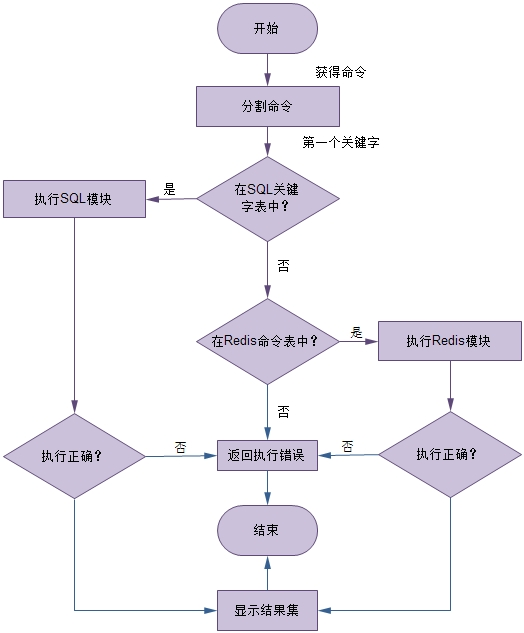
\includegraphics[width=0.9\textwidth]{Selector}
\caption{选择处理模块的流程设计}\label{fig:Selector}
\vspace{\baselineskip} %表示图与正文空一行
\end{figure}

\section{性能优化设计}
\begin{enumerate}[label=(\arabic*)]
\item{根据系统不同需求,修改redis.config中的参数}
\end{enumerate}

\section{本章小结}
本章在第三章、第四章的基础上对系统进行了详细设计。首先,在系统开发之前,对系统的开发规范,包括目录规划进行了规定。重点介绍系统功能模块的详细设计及其流程,紧接着对性能优化等方面进行了设计。

%%% 第六章 项目中期检查系统实现  %%%
\chapter{系统实现}
% 6.1   系统界面实现  20
% 6.2   系统框架整合实现    23
% 6.3   系统功能模块实现    23
% 6.4   本章小结    23

\section{系统界面实现}
本系统中所有的界面均采用PyQT4进行设计,如%%%TODO
所示

\section{系统框架整合实现}

\section{系统功能整合实现}

\section{本章小结}
本章对系统实现中的核心技术进行了深入的介绍,包括了框架整合技术现实、系统功能模块实现,最后给出了系统实现的部分功能模块界面。


%%% 第七章 系统测试    %%%
\chapter{系统测试}
% 7.1   系统测试    24
% 7.1.1 数据正确性测试 24
% 7.1.2 系统功能测试  24
% 7.2   本章小结    24
\section{系统测试}
软件测试是软件开发整个生命周期中对软件质量进行有效控制的重要手段,是在规定的条件下对程序进行操作,以发现程序错误,衡量软件质量,并对其是否能满足设计要求进行评估的过程。实际的软件工程实践证明,让对软件思想有深刻理解的工程师进行软件测试,可以大幅度的提高软件质量。

\subsection{正确性测试}
正确性是指软件按照需求正确执行任务的能力,无疑是第一重要的软件质量属性。如果软件运行不正确,将会给用户造成不便甚至损失。技术评审和测试的第一关都是检查工作成果的正确性。
正确性说起来容易做起来难。因为从“需求开发”到“系统设计”再到“实现”,任何一个环节出现差错都会降低正确性。机器不会主动欺骗人,软件运行出错通常都是人造成的,所以不要找借口埋怨机器有毛病。开发任何软件,开发者都要为“正确”两字竭尽全力。

本系统通过随机添加删除查找数据的方式,将对应的结果集和MySQL 5.5进行对比,从而对系统的正确性进行测试。

\subsection{性能测试}
性能测试是对软件性能的评价。简单的说,软件性能衡量的是软件具有的响应及时度能力。因此,性能测试是采用测试手段对软件的响应及时性进行评价的一种方式。对数据库系统而言,命令的响应处理速度是一个很重要的关键点,所以本系统采用对数据库进行批量读写的操作来测试读写速度,下文通过同样的手段测试关系型数据库代表Mysql 5.5的性能,并与本系统作比较。
%%% TODO %%%

\section{性能对比} %%% 自己加的,与MySQL 5.5对比

\section{本章小结}
本章对系统进行测试,主要进行系统的数据正确性测试与性能测试。

% 第八章 总结    25
% 8.1 完成的工作 25
% 8.2 存在的问题及下一步工作   25
\chapter{总结}
\section{完成的工作}

\section{存在的问题及下一步工作}

% \makeatother
\backmatter

%%%%%%%%%% 参考文献 %%%%%%%%%%
\bibliography{references/reference}
\nocite{*}                                   % 若将此命令屏蔽掉,则未引用的文献不会出现在文后的参考文献中。

%%%%%%%%%% 致谢 %%%%%%%%%%
% !Mode:: "TeX:UTF-8"

%\titlecontents{chapter}[2em]{\vspace{.5\baselineskip}\wuhao\hei}
%{\prechaptername\CJKnumber{\thecontentslabel}\postchaptername\qquad}{}
%{\hspace{.5em}\titlerule*[10pt]{$\cdot$}\wuhao\contentspage}
\chapter{\heiti\bfseries{致谢}}

浙江工业大学本科生毕业论文~\LaTeX~模板主要参考以下内容:
\begin{itemize}
  \item 天津大学本科生毕业论文
  \item 哈尔滨工业大学~PlutoThesis~硕博士学位论文模板
  \item 武汉理工大学学位论文~WHUTThesis~模板
  \item 中科院~CASthesis~模板
  \item 浙江大学~cs\_zjut\_theis~模板
  \item 上海交通大学毕业论文Latex模板
\end{itemize}

\vspace*{1em}

衷心感谢导师~XXX~(职称)对本人的精心指导。他/她的言传身教将使我终生受益。

感谢~XXX~教授,以及实验室全体老师和同窗们的热情帮助和支持!




            % 致谢

%%%%%%%%%% 附录 %%%%%%%%%%
\appendix
% !Mode:: "TeX:UTF-8"
%
% XXX refactor 暂时当静态页面处理
% 
\chapter{附录}

\phantomsection

\addcontentsline{toc}{section}{附录1 毕业设计文献综述}
\addcontentsline{toc}{section}{附录2 毕业设计开题报告}
\addcontentsline{toc}{section}{附录3 毕业设计外文翻译}
\hspace*{7.0mm}
\hspace*{4.0mm}
\begin{minipage}[t]{95mm}
    \heiti\bfseries{
    \sectionmark{附录1 毕业设计文献综述}
    附录1 毕业设计文献综述

    \vspace*{7.0mm}

    \sectionmark{附录2 毕业设计开题报告}
    附录2 毕业设计开题报告

    \vspace*{7.0mm}

    \sectionmark{附录3 毕业设计外文翻译}
    附录3 毕业设计外文翻译}
\end{minipage}


            % 附录

% 以下注释内容需放在第一个附录tex文件的头部,放在主文件里会造成“附录”两字单独成页。
%\setlength{\parskip}{18pt}
%\chapter*{\centering\hei\xiaoer{附\qquad 录}}
%\setlength{\parskip}{18pt}
%\setlength{\parskip}{0pt}

\end{document}                                  % 结束全文
